\documentclass{sigchi}



% Load basic packages
\usepackage{balance}  % to better equalize the last page
\usepackage{graphics} % for EPS, load graphicx instead
\usepackage{times}    % comment if you want LaTeX's default font
\usepackage{url}      % llt: nicely formatted URLs

% llt: Define a global style for URLs, rather that the default one
\makeatletter
\def\url@leostyle{%
  \@ifundefined{selectfont}{\def\UrlFont{\sf}}{\def\UrlFont{\small\bf\ttfamily}}}
\makeatother
\urlstyle{leo}


% To make various LaTeX processors do the right thing with page size.
\def\pprw{8.5in}
\def\pprh{11in}
\special{papersize=\pprw,\pprh}
\setlength{\paperwidth}{\pprw}
\setlength{\paperheight}{\pprh}
\setlength{\pdfpagewidth}{\pprw}
\setlength{\pdfpageheight}{\pprh}

% Make sure hyperref comes last of your loaded packages, 
% to give it a fighting chance of not being over-written, 
% since its job is to redefine many LaTeX commands.
\usepackage[pdftex]{hyperref}
\hypersetup{
pdftitle={HuRich\_Final\_Writeup},
pdfauthor={LaTeX},
pdfkeywords={},
bookmarksnumbered,
pdfstartview={FitH},
colorlinks,
citecolor=black,
filecolor=black,
linkcolor=black,
urlcolor=black,
breaklinks=true,
}

% create a shortcut to typeset table headings
\newcommand\tabhead[1]{\small\textbf{#1}}


% End of preamble. Here it comes the document.
\begin{document}

\title{stressSpectra: QUANTIFYING WELLBEING THROUGH DICHOTOMOUS KEY SEARCHING }

\numberofauthors{2}
\author{
  \alignauthor Kevin Hu\\
    \affaddr{MIT Media Lab}\\
    \affaddr{75 Amherst St}\\
    \email{kzh@media}\\
    % \affaddr{Optional phone number}\\
  \alignauthor Travis Rich\\
    \affaddr{MIT Media Lab}\\
    \affaddr{75 Amherst St}\\
    \email{trich@media}\\
    % \affaddr{Optional phone number}\\    
}

\maketitle

\begin{abstract}
Many experiments in need of a stress measurement employ a Likert scale, or more generally a discrete self-evaluation from 0 to N, to measure subject affect (happiness, stress, etc). While this form of self-evaluation is simple to understand and easy to use for both researchers and test subjects, it possesses numerous flaws that we find exceedingly troublesome. The arbitrary nature of the chosen number or definition of 'strongly' means that it can be frustratingly unclear what a person's response specifies. A subject's response can be biased by preconceived notions of appropriate answers and each subject has a different internal distribution for a given question. Furthermore, the result of such scale gives little insight into the human condition - life is much more complex than a 1-5 scale. We have built and tested a system that using simple binary comparison votes to build a spectrum of stressful events that is personalized to the individual. This spectrum of events can then be used to gain an understanding of a person's current stress level. We believe this tool provides a richer and more powerful platform for understanding, comparing, and analyzing the dynamics of stress in a person's life. 
\end{abstract}


\section{Introduction}

Our stress levels dictate much of our day-to-day experience \cite{kanner1981comparison} \cite{levy1997relationship}. How stressed we feel at any given moment can impact our performance, our health, and our outlook on life \cite{delongis1988impact} \cite{bolger1989effects}. For these reasons, it is no surprise that there is great interest in being able to measure and analyze a person's level of stress. This of course is a tricky problem as there is no explicit physical phenomenon to measure. Stress manifests itself in a wide and diverse set of ways. Many past attempts to measure stress take an approach that is either overly simple or frighteningly clinical. In order to provide a richer and friendlier means of understanding a person's stress (and its inherent diversity) we have built stressSpectra. The tool is a web application that allows a user to generate a personalized spectrum of stressful events. This spectrum can then be used to understand a person's stress level at a given moment (and thus over time) or compare their stress spectrum to others to reveal idiosyncrasies. 


\section{Existing Methods}
Existing methods for self-reporting subjective stress, excluding physiological methods, fall into four categories. In first two interview methods and journaling methods. In the first category are questionnaires in which a subject reports stress level in terms of a value on a numeric scale. The Likert psychometric scale is a common example \cite{maurer1998comparison}. The second category consists of questionnaires in which a subject marks which events she has experienced. Examples include the Holmes and Rahe scale, the Perceived Stress Scale, and the Daily Stress Inventory \cite{CSHSquestionnaires} \cite{holmes1967social} \cite{brantley1988convergence}. 

Interview and journaling methods are versatile and highly dimensional. However, because of their free-form and ad-hoc nature, these methods are difficult to scale, and the data produced from these methods are difficult to analyze rigorously \cite{howtomeasureinhumans}.

Likert-like questionnaires have the advantage of being quick to create and use, and produce data which is easy to analyze and analytically rigorous \cite{bland1997statistics}. Because of these advantages, Likert-like methods are common both in psychometric studies and other fields. However, these methods face major shortcomings in terms of their bias and validity. First, they do not account for different underlying distributions for each subject. For example, some subjects may hesitate to report extremes. Second, they usually only allow for discrete inputs (e.g. How stressed are you from 1-5) whereas the metric in question is usually continuous.

Event-based questionnaire forms can further be classified by the time-scale in question. Some forms revolve around life events, while others are concerned with daily events or chronic stress \cite{macarthurResearch}. Regardless of the time scale, these questionnaire-like forms, while having the advantage of tying stress to specific, relatable events, also face major limitations. For instance, these forms are dependent on subjects having experienced a certain list of events, and therefore are demographic-dependent. Further, these forms, similar to the Likert-like forms, do not account for differences between individuals. For instance, 'singing in public' may be extremely stressful for one subject while being pleasurable for another. Lastly, these forms are lacking from an experience point-of-view: they require a large, tedious time investment from a subject.


\section{Proposed Design Additions}
As stated in the previous section, while the Likert-like questionnaire and event-based questionnaire are quantitative and analytically tractable, in contrast with the interview and journalling methods, they contain two major flaws. First, they do not account for varying distributions between subjects. Second, they oversimplify the continuous nature of stress.
Therefore, in creating stressSpectra, we hope to create a tool that calibrates a stress scale peresonalized to a given subject, is dynamic and adjusts to new formation, and treats stress events in a continuous manner.
With these continuous, dynamic, personalized scales in place, then we aimed to add features which are supplementary, but potentially useful, to the subjects. For instance, stressSpectra contains a feature allowing a subject to compare the distribution of her stress events to the global distribution. Lastly, we aimed to make the experience more fun than a pen-and-paper test.

\section{Architecture}
stressSpectra is designed as a web-accessible application. Most generally, we can split the design elements into two groups: frontend and backend. The frontend encompasses everything the user sees and all of the interaction schema. The backend encompasses the data management, site-serving technologies, and analysis code. 

The backend is a contained module which stores the varying stress content, accepts votes comparing these stress content, provides random contestants (i.e. stress events), and makes analyzed results accessible via HTTP requests. This functionality is all built on top of Flask \cite{flask} - a Python-based microframework. The framework is hosted on Amazon's Elastic-beanstalk service, which allows for dynamic scaling based on site usage and demand. All votes are received and stored in a single global pool. Votes are then processed to calculate global results and an individual's results separately. Once processed, the vote is marked so that all future results can be calculated without re-processing old votes. This allows us to update results very quickly and with low computational-overhead. 

The frontend is built on top of Angular \cite{angular} - a javascript framework. The frontend manages the calls to the backend API and dictates the interactions and experience of the user. All front-end code is hosted statically on Amazon's S3 service. The user-experience is separated into 3 main sections: Calibrate, Measure, and Compare. 


\section{Calibrating Baseline}
The calibrate section provides a simple interface posing the question 'Which seems to be more stressful?'. The user is then presented with three options: two  situations or an 'I don't know' button. The user clicks either one of the stressful situations or the 'I don't know' button signaling their subjective interpretation of which event seems more stressful. There are a total of 250 situations in the system. Theoretically, we would need N*log(N) votes (or 1992 votes given N=250) to reach a completely mapped spectrum. However, given our processing algorithm, based off the Trueskill ranking algorithm \cite{herbrich2006trueskill}, we find that acceptable results are seen around 100 votes, and mostly converged results are seen around 1000 votes. This is due to the algorithm's ability to infer data from past votes. It interprets each vote, and thus the ranked scores, as non-independent events.
\begin{figure}[!h]
\centering
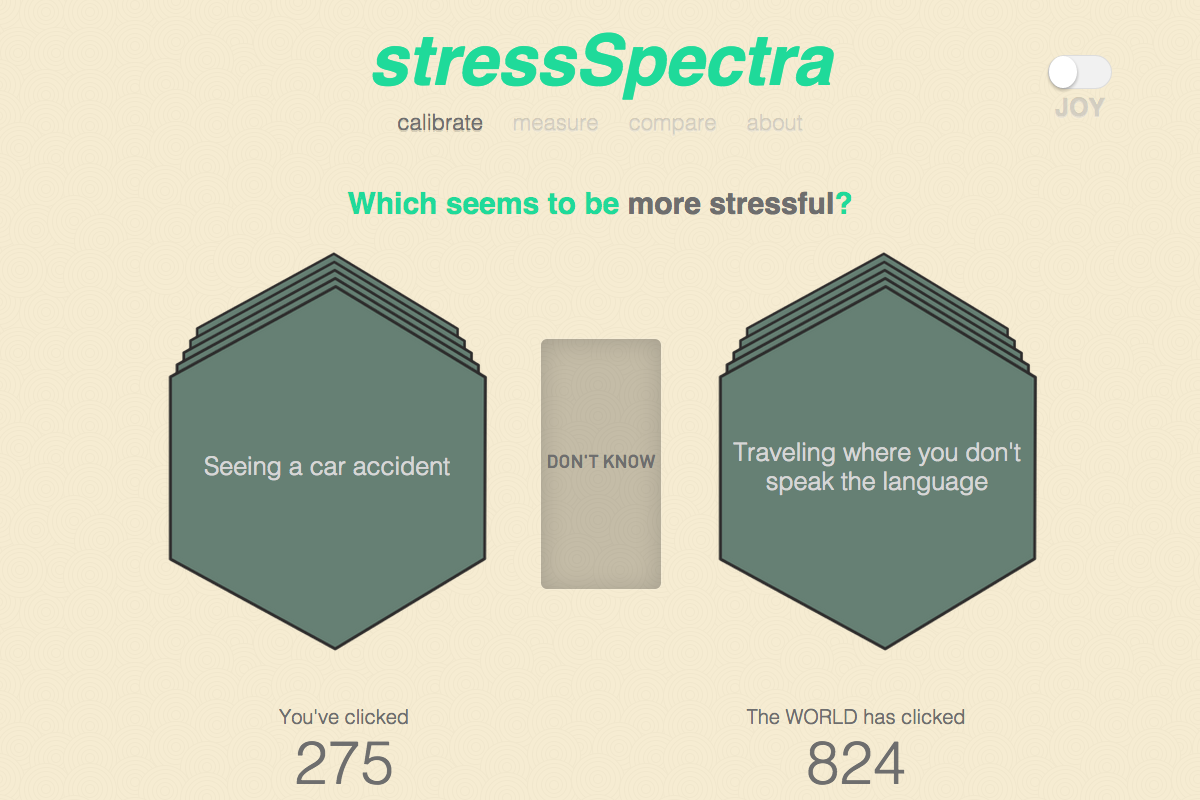
\includegraphics[width=0.9\columnwidth]{calibrate}
\caption{stressSpectra Calibration screen}
\label{fig:calibrate}
\end{figure}

The experience is designed such that after 5 votes, the user is presented with a review screen that serves as a breath between the cycles of clicking. A 'Joy Mode' feature is added which allows us to incorporate silly and playful interface elements into the design of the project. In the Calibrate section, Joy mode toggles a series of animated cat GIFs on the review screen. The GIFs give the user a moment of enjoyment and motivates more voting for the sake of seeing a new set of adorable, cute cat GIFs. Given that the system requires many votes, these playful interventions serve as a way to break the monotony of dozens and dozens of comparison clicks.

\section{Measuring State}
The Measure section is designed to find a user's current level of stress by comparing various stressful situations to their current level of perceived stress. The page takes a user's spectrum of situations (from most stressful to least stressful) and traverses the spectrum in a binary-search pattern by asking the user if they feel more or less stressed than the presented situation. For example, a user is asked, 'Do you feel more, less, or equally stressed as you would if you had an assignment overdue?'. Depending on the vote, a user is presented with a new question repeated on a subset of their spectrum.
\begin{figure}[!h]
\centering
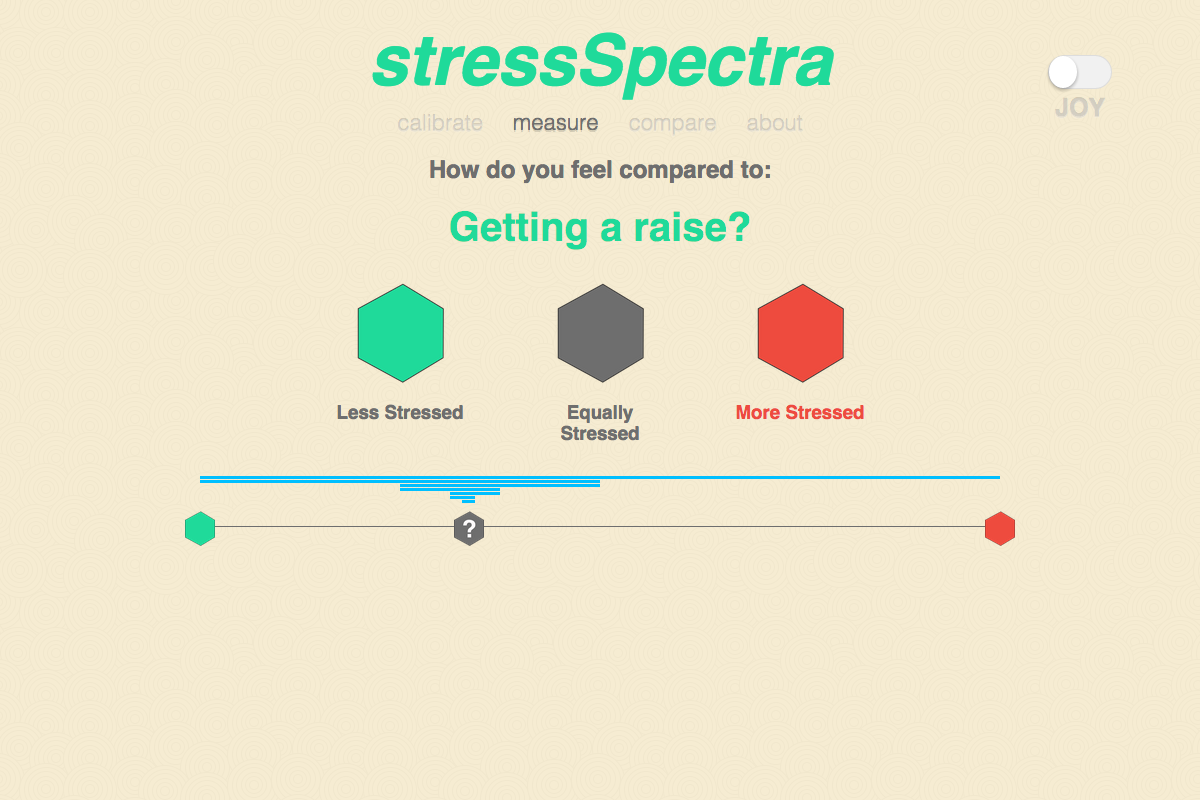
\includegraphics[width=0.9\columnwidth]{measure1}
\caption{stressSpectra Measure screen}
\label{fig:calibrate}
\end{figure}

A user's resultant state is saved for future comparisons. Upon resolving the current state, all previous states are visually presented so that the user can see how their stress state has changed over the course of time.  
\begin{figure}[!h]
\centering
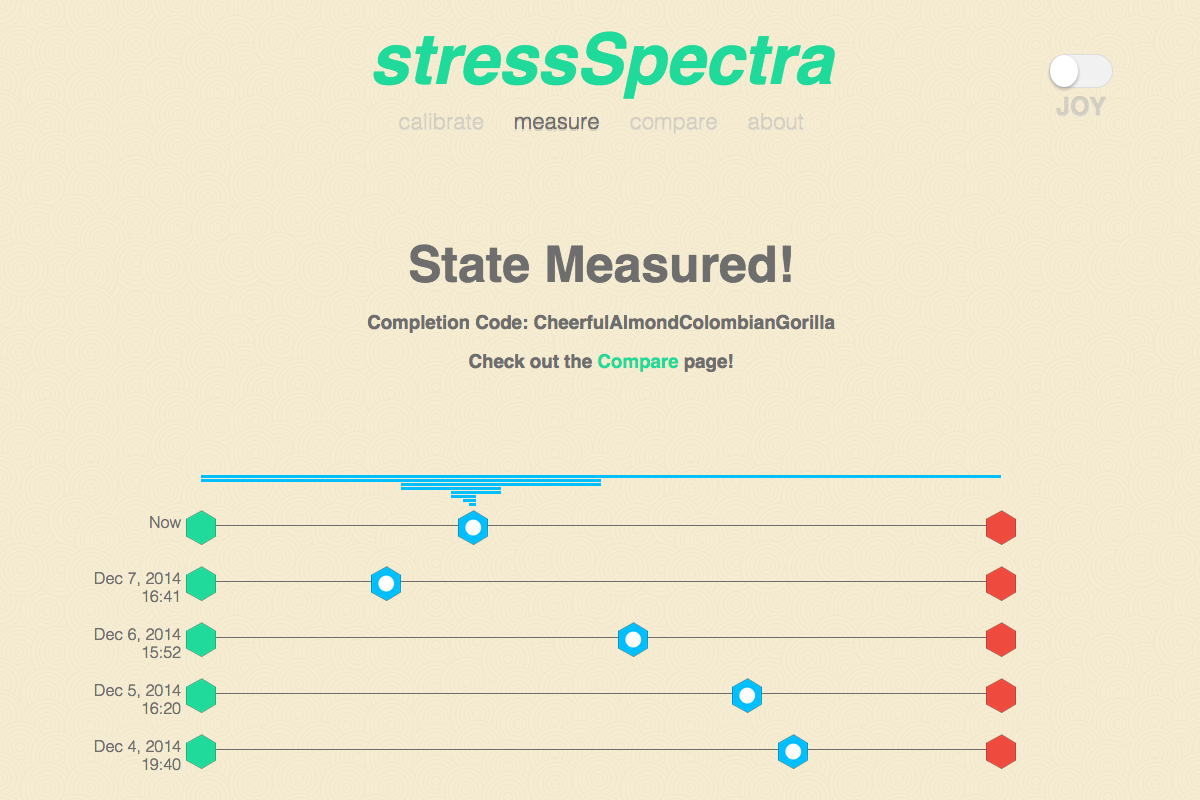
\includegraphics[width=0.9\columnwidth]{measure2}
\caption{Successful measurement of a stress state}
\label{fig:measure}
\end{figure}

\section{Comparing Results}
The Compare section allows a user to compare their stress spectrum to the globally averaged spectrum. That is, it compares the spectrum as calculated from the votes cast by a specific user to the spectrum calculated from all votes in the entire system.
\begin{figure}[!h]
\centering
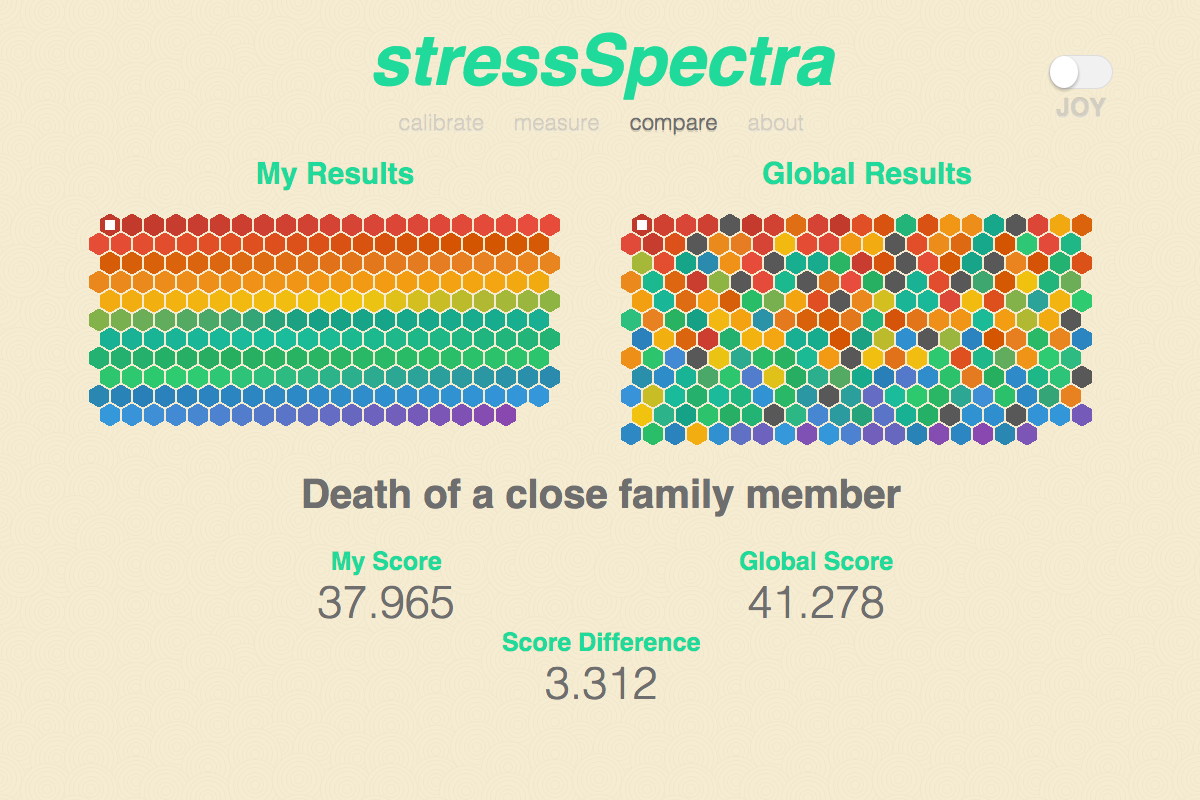
\includegraphics[width=0.9\columnwidth]{compare}
\caption{stressSpectra Compare screen}
\label{fig:compare}
\end{figure}

The user's spectrum is ordered from most to least stressful. Each stress situation is given a color based on it's position in the spectrum. A rainbow is used where red denotes more stressful events and purple denotes less stressful events. The global results are similarly plotted from most to least stressful, but the colors are chosen such that they match the events of the user's spectrum. That is, a given stress situation only has a single color, as dictated by its ordering in the user's spectrum. This allows for fast comparison of where a user's perception of the stress associated with a given event strongly differs from the global consensus. 

\section{Evaluation}
To evaluate stressSpectra we built a user study and distributed it to a set of people (N=10). The study has each participant complete three different stress measurements: 1) a simple 1-10 self-report of stress, 2) a Holmes and Rahe stress test, and 3) a stressSpectra profile. Each participant is then also asked to provide qualitative feedback on the experience. 


Figure \ref{fig:rangeuse} shows histograms of the measured scores for each test. Some first observations of the distribution patterns are interesting. The Likert scale shows a bifurcation and is heavily weighted towards the upper end of the spectrum. The Holmes and Rahe distribution, which has a minimum score of 0 and a maximum possible score of 1400, shows a very strong bias towards the lower end of its range. The stressSpectra distribution is more similar to a Gaussian distribution with a mean near the middle of the full range. 
\begin{figure}[htb]
\centering
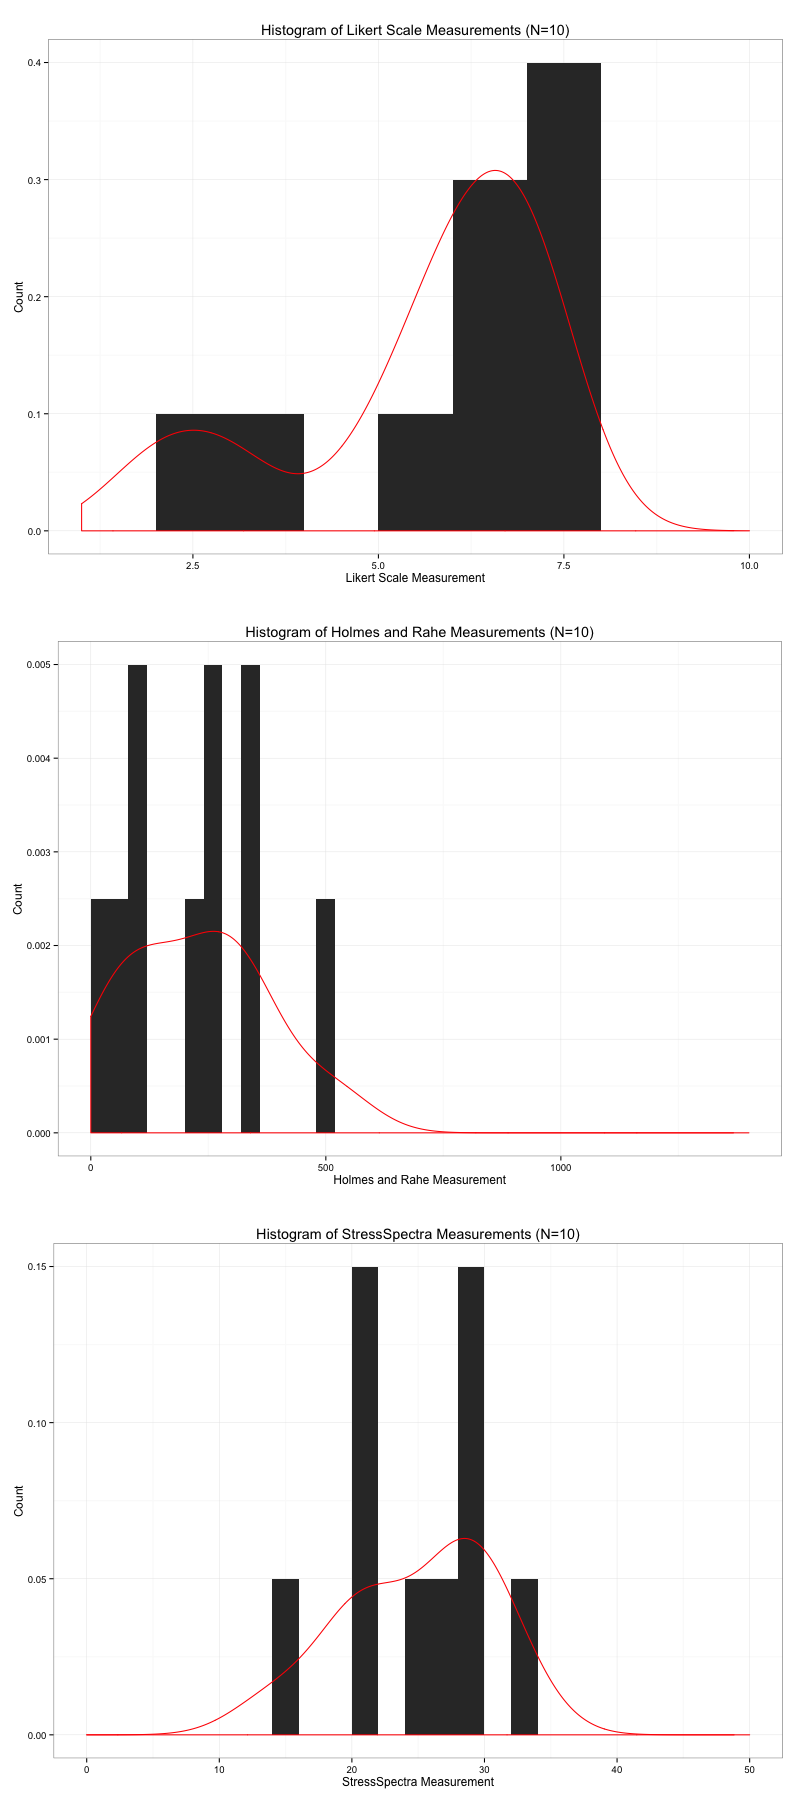
\includegraphics[width=0.9\columnwidth]{rangeUse}
\caption{Histogram of measurements for each stress test.}
\label{fig:rangeuse}
\end{figure}


Figure \ref{fig:correlation} shows a matrix with the correlation values for each pair of results. As is also shown in Figure \ref{fig:evalreg}, the Holmes and Rahe measurements are negatively correlated with the Likert and stressSpectra measurements. The Likert and stressSpectra measurements are 69\% correlated with a p-value of 0.028.

\begin{figure}[h!]
\centering
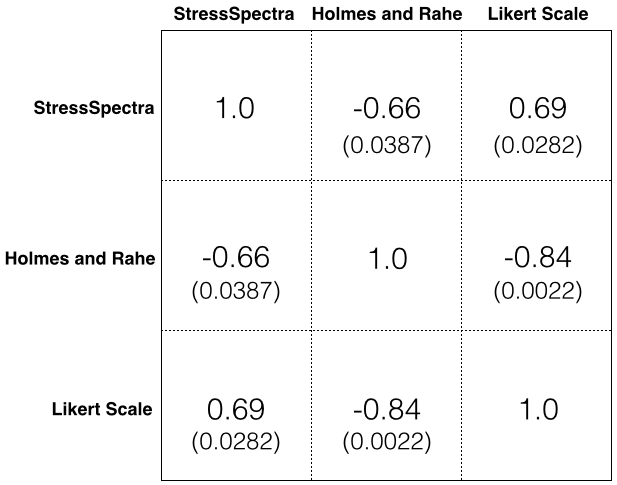
\includegraphics[width=0.9\columnwidth]{correlation}
\caption{Matrix showing correlation values for each pair of tests.}
\label{fig:correlation}
\end{figure}


Figure \ref{fig:evalreg} shows the linear regression calculation between all pairs of measurements. We can see that the stressSpectra and Likert scales are positively correlated. Surprisingly, the Holmes and Rahe measurements are negatively correlated to both the Likert and stressSpectra measurements. The conclusions to be made could either be that the test is inaccurate or, more interestingly, that the Holmes and Rahe measurement (which deals more with long-term life events) is an indicator for people's ability to cope with daily in-the-moment stress (as measured by Likert and stressSpectra). Thus, people with high Holmes and Rahe scores have learned to cope well with stress, leading to lower stress readings in their day-to-day life. 
\begin{figure}[h!]
\centering
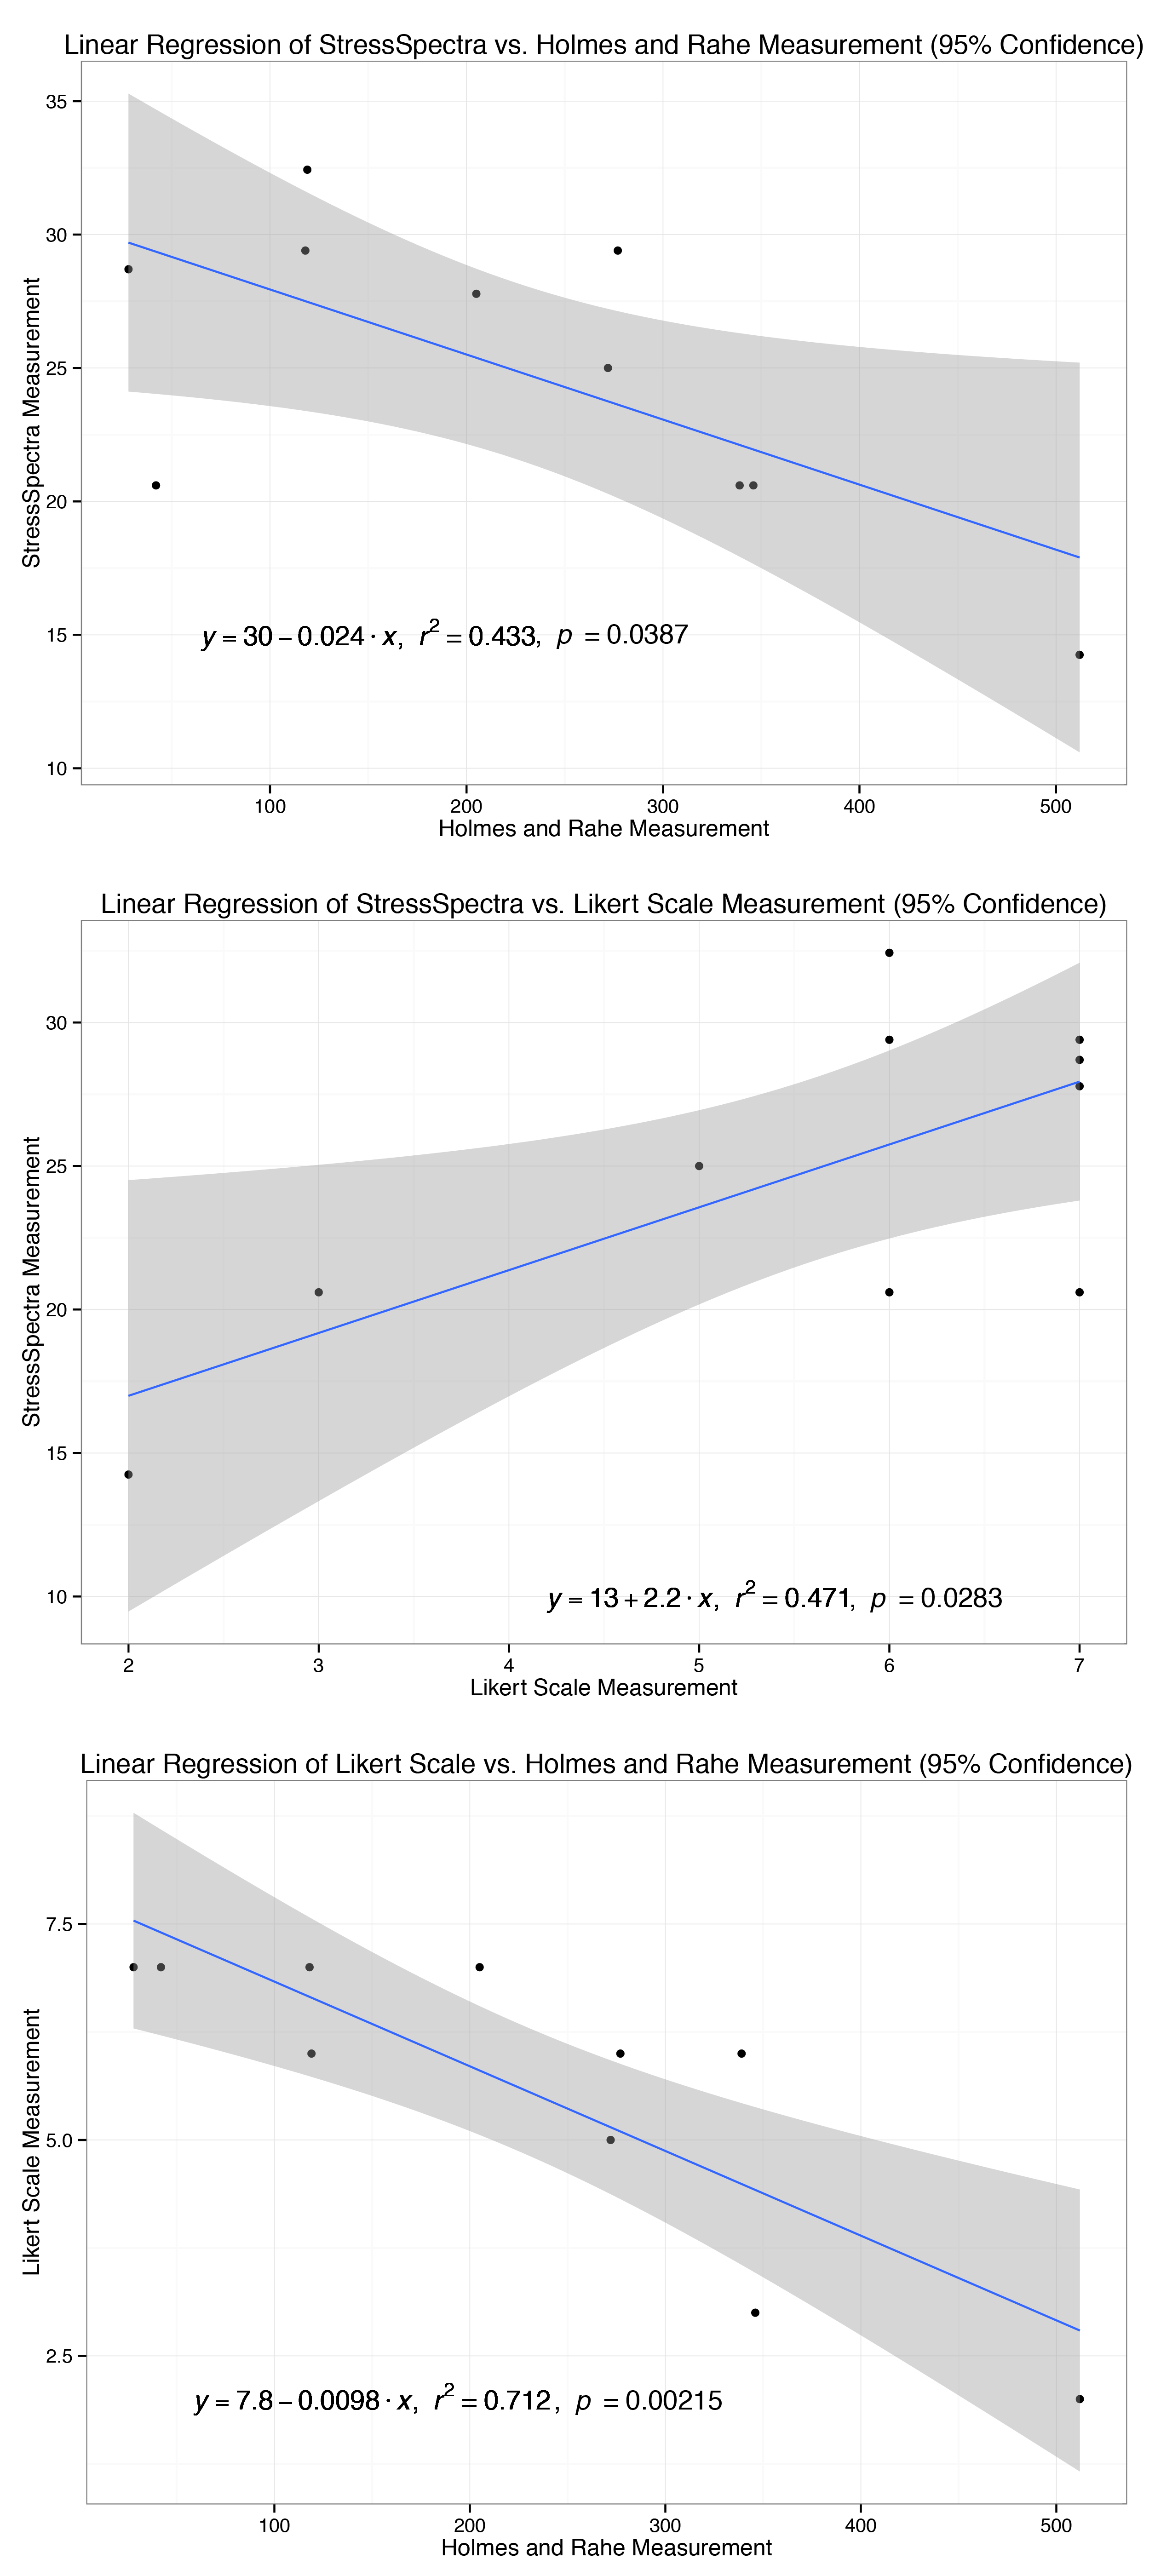
\includegraphics[width=0.9\columnwidth]{evalRegression}
\caption{Linear regression comparing the measured scores of the various tests.}
\label{fig:evalreg}
\end{figure}





\section{Contributions}
We find the contributions of stressSpectra to fall into three categories: 1) the exploration of a globally dynamic set of stress stimuli, 2) the dynamic personalization of stress events and their weight, and 3) the design of an interface for more playful and enjoyable engagement with stress measurements.

Through personal experience and qualitative feedback, we found that the idea of a globally dynamic set of stress stimuli allowed for an enhanced ability to relate to the stressful events of everyday life across different demographics. That is, for many people, having a dead cellphone is more stressful than becoming a parent because many people have not yet become parents. By using a dynamic set of stimuli, we open the set to include small daily occurrences in addition to major life events. 

Such comments also hold true for the personalization of stress events and their impact. How a person perceives an unplanned pregnancy is likely to change drastically over the course of their life. Thought we did not have time to perform a longitudinal study on any meaningful timescale, the personalized spectrum approach does allow the work to remain relevant for people of different ages. 

The largest effect we saw in the interface design was the inclusion of the 'Joy Mode' button. Despite the simple and irrelevance of animated GIFs and smiley faces to the task at hand, the little moment of happiness and distraction were immediately resultant in smiles and what appeared to be an enhanced enthusiasm to get through the next set of votes. While we were only able to observe a small set of the evaluation participants, we think that the inclusion of such playful elements give the project a less clinically-serious feel which is important for the sake of making stress measurement and discussion a part of everyday healthy life, as opposed to a symptom that must be medically treated. 

\section{Conclusion}
We have explored a way to make personalized, dynamic stress measurements. The quantitative evaluation, while limited in participant size showed correlation between the stressSpectra measurements and typical Likert-scale measurements. The stressSpectra results also demonstrated a less bifurcated spectrum of scores and results, though it was difficult to make concrete quantitative conclusions from the small population size.

The qualitative feedback from users of the application suggested that while the extremes held true (the very stressful and very non-stressful events were accurate) the middle range of results were less than ideal. This indicates a need to either 1) collect more votes, or 2) more intelligently produce our rankings. Further qualitative feedback was positive and suggested a high level of engagement with the application. This engagement seems to be largely driven by 'Joy mode' which seemed to add a playful and engaging aspect to the site that other stress measurements lack. 


Future steps we envision designing a more intelligent system that can further reduce the number of required votes. We find that giving quick results is key to generating an experience that people stick with. Furthermore, we can see additional features on the Compare page having much utility. Enabling users to compare to other users pr sets of users (say, all users in a given state or age-range), in addition to the global range, would provide a richer tool for understanding one's own idiosyncrasies. Importantly, with more time, we also see value in launching a wider study around the evaluation metrics with a much larger sample size and diversity of tests.



\balance


\bibliographystyle{acm-sigchi}
\bibliography{myBib}
\end{document}
